%% LyX 2.0.2 created this file.  For more info, see http://www.lyx.org/.
%% Do not edit unless you really know what you are doing.
\documentclass[english]{article}
\usepackage[T1]{fontenc}
\usepackage[utf8]{inputenc}
\usepackage[a4paper]{geometry}
%\geometry{verbose,tmargin=3cm,bmargin=2cm,lmargin=2cm,rmargin=3cm}
\setlength{\parskip}{\medskipamount}
\setlength{\parindent}{0pt}
\usepackage{amsthm}
\usepackage{amsmath}
\usepackage{amssymb}
\usepackage{graphicx}
\usepackage{setspace}
\usepackage[bottom]{footmisc}
\onehalfspacing

\makeatletter

%%%%%%%%%%%%%%%%%%%%%%%%%%%%%% LyX specific LaTeX commands.
%% Because html converters don't know tabularnewline
\providecommand{\tabularnewline}{\\}
%% A simple dot to overcome graphicx limitations
\newcommand{\lyxdot}{.}


%%%%%%%%%%%%%%%%%%%%%%%%%%%%%% Textclass specific LaTeX commands.
\numberwithin{equation}{section}
\numberwithin{figure}{section}

\@ifundefined{date}{}{\date{}}
%%%%%%%%%%%%%%%%%%%%%%%%%%%%%% User specified LaTeX commands.
\usepackage[english]{babel}
\usepackage{amsfonts}
\usepackage{array}
\usepackage{hhline}

\makeatother

\usepackage{babel}
\begin{document}

\title{a4a kick-off meeting report\\
28th February to 2nd March, 2012\\
JRC, Ispra, Italy }

\maketitle
\noindent \begin{center}
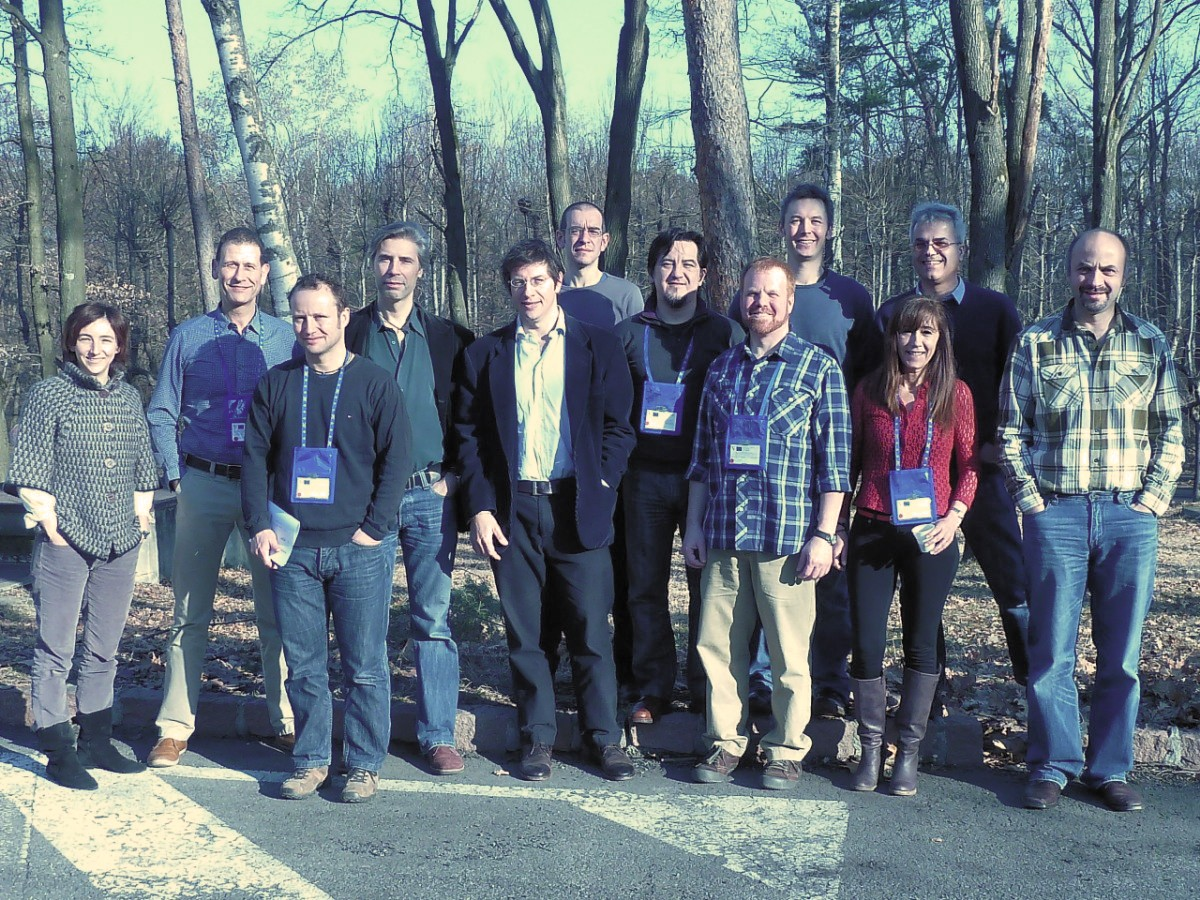
\includegraphics[width=0.9\textwidth]{img-1}
\par\end{center}

\pagebreak{}


\section{Introduction}

The implementation of the 2009 revision of the DCF%
\footnote{Data Collection Framework (2008/949/EC)%
} generated the obligation to collect a large amount of information
for all stocks being subject to fisheries exploitation. Based on the
regulation there are 250+ stocks for which some kind of biological
information must be collected. Most of these stocks will have in the
future, $\sim$2020, time series of exploitation data more than 10
years long, although the biological information will most likely
be limited due to the high human resources requirements to process all the samples collected.
These stocks (will) have a moderate amount of information and won't
fit into the \textquotedbl{}data poor\textquotedbl{} stock definition.
In addition, due to the large number of these stocks, it is not logistically
feasible to run on all of them complex data eager models that require a high level
of expertise. What is required is a robust methodology
that allows the assessments of a large number of stocks by stock assessment 
experts with distinct backgrounds. 

Having stock assessment and advisory methods to apply to a large number
of moderate data stocks, raise interesting challenges and creates
opportunities worth exploring. For example, approaching stock assessment
as a data generating engine, having a common stock assessment methodology
or analyzing massive\footnote{In the sense of analyzing a large number of stock metrics, 
which will open the possibility of using methods like data mining or other "big data" methods.} 
stock assessment results, open the possibility of issuing advice for more species in a multifleet, multispecies framework
and promotes comparative analysis. 

As scientists it is important to think ahead and start developing
such methodologies. JRC following it's mission of anticipating policy
implementation issues decided to move forward with the ``Assessment
for All'' (a4a) initiative, aiming to: 
\begin{enumerate}
\item develop an assessment method targeting stocks that have a reduced
knowledge base on biology and moderate time series on exploitation
and abundance; 
\item trigger the discussion about the problem of massive stock assessment;
\item build capacity on stock assessment and fisheries management advice.
\end{enumerate}
The initiative has a web repository where all the presentations, reports,
code and data can be found%
\footnote{https://github.com/ejardim/a4a%
}.


\subsection{Objectives and organization}

The kick-off meeting of the initiative took place between 29/February
and 02/March of 2012 at the JRC headquarters in Varese, Italy, chaired
by Ernesto Jardim (JRC/EC), with the following terms of reference:
\begin{enumerate}
\item overview of current worldwide needs for fisheries advice; 
\item brief review of available stock assessment methods of relevance to these stocks; 
\item possible ways to make stock assessment more robust in the context of providing management advice; 
\item identify necessary modules to build a simulation for advice framework; 
\item discuss the direction and progress of the initiative. 
\end{enumerate}

The agenda of the meeting can be found in Annex I.

\subsection{Participants}

\begin{tabular}{rrl}
\hline 
Name &  & Affiliation\tabularnewline
\hline 
Andrew Cooper &  & Simon Fraser University (CA)\tabularnewline
Chato Osio &  & Joint Research Center (EC)\tabularnewline
Einar Nielsen &  & Danish Technical University (DK)\tabularnewline
Ernesto Jardim (chair) &  & Joint Research Center (EC)\tabularnewline
Finlay Scott &  & Centre for Environment, Fisheries \& Aquaculture Science (UK)\tabularnewline
Gary Carvalho &  & Bangor University (UK)\tabularnewline
Iago Mosqueira &  & Joint Research Center (EC)\tabularnewline
Jann Marthinson &  & Joint Research Center (EC)\tabularnewline
Jose de Oliveira &  & Centre for Environment, Fisheries \& Aquaculture Science (UK)\tabularnewline
Leire Ibaibarriaga &  & AZTI Tecnalia (ES)\tabularnewline
Manuela Azevedo &  & Portuguese Institute for Sea and Atmosphere (PT)\tabularnewline
Ruben Roa &  & AZTI Tecnalia (ES)\tabularnewline
\hline 
\end{tabular}


\subsection{Background information}

A general introduction to the subject, aims and objectives was carried out by Ernesto Jardim to open
the meeting, followed by a set of presentations of reports and other
initiatives, that could contribute to the progress of the work\footnote{All the presentations
are available on the a4a repository.}. Manuela
Azevedo presented the recent outcomes of the ICES WKLIFE, the south
hemisphere initiative on Management Strategies Evaluation (MSE) report was presented by Iago Mosqueira,
the GFCM workshop on Elasmobranchs was presented by Chato Osio and
Andrew Cooper presented the management system implemented in the USA
after the revision of the Magnuson-Stevens act. 

\section{Outcomes}

The ToR and agenda were followed loosely to allow for discussions
and brain storming. 

The overall objective was to consolidate ideas regarding the initiative's
aims, expectations and operationalization. It was critical to better
define the problem the initiative is attempting to contribute to,
discuss the range of solutions available and define which ones the
initiative should pursue. In that sense the meeting was successful
and the objectives were achieved. 

The discussions gave rise to the definition of a ``moderate data
stock'', a major step to understand where the initiative intends
to contribute. The issue of introducing genetics in fisheries management
was discussed and several clarifications were made, as well as the
identification of promising areas of convergence between fisheries
modeling and genetics. Another issue to be grounded was the assessment or population
model(s) to be explored, for which a set of characteristics were defined
while leaving open the exact framework to be used. A further step
was taken by designing the type of MSE
the initiative will promote/develop as a standard advice methodology
for these type of stocks. In a more pragmatic setting the group loosely
defined an initial simulation experiment to be carried out and a set of issues
to be tested. Additionally the group discussed the a4a operationalization.


\section{Conceptual framework}


\subsection{Moderate data stock}

The group discussed the characteristics of a ``moderate data stock''
in terms of data types and availability, and agreed on the following definition.

A moderate data stock has at least data on:
\begin{itemize}
\item nominal effort, 
\item volume of catches in weight (which should include landings and discards), 
\item length structure of the catches (based on selectivity studies or
direct observations),
\item information-based maturity ogive (parameters are not educated guesses
but based on information),
\item information-based growth model (parameters are not educated guesses
but based on information),
\item length-weight relationship,
\item index of abundance (the type of index is left open, it
could be a scientific survey or a commercial CPUE series),
\item length structure of the index of abundance (based on selectivity
studies or direct observations)
\end{itemize}
The length of the time series required is not considered to be of major importance, as it will
depend on the species' longevity.


\subsection{Genetics}

While there is general agreement that genetic approaches can support
fisheries management relevant issues, a clear need persists to clarify
how and where exactly genetic analysis could contribute to fisheries
management advice and stock dynamics modeling, particularly when
applied in a routine context. 

To start with, a clear distinction must be made between the usage
of genetics for control and enforcement, like determining the origin
of individuals or species/stock mis-identification, and the usage
of genetic indicators or metrics for modeling purposes, which was
the aim pursued in the discussions taking place during this meeting. 

The discussions focused on three distinct themes: stock identification,
risk indicators, and total biomass/abundance estimation. 

Stock identification is the most promising area of convergence, and
the application of genetics for this purpose seems most readily available
as a routine approach in fisheries management: there exist already
a number of examples where genetic stock identification (GSI) is used
and the genetic analysis applied is robust and relatively easy to
perform. When applying GSI, the major effort arises through the need
to establish a baseline, which depends on finding the allele composition
that separate the stocks/populations/groups. Better definitions of
stock boundaries, estimates of migration rates, Harvest Control Rules
(HCRs) based on the percentage of certain groups on the catch, etc,
can all be plugged into stock dynamics modeling or management procedures
simulations. Following these ideas the group discussed and suggested
a non-exhaustive set of questions that could be tested on a MSE framework: 
\begin{itemize}
\item What if there are two subpopulations with distinct biological characteristics
managed as a single stock; 
\item Which kind of HCR can be applied to a group of species based on knowledge
of their percentage on the catch;
\item How robust is the management procedure to departures from the closed
population stock assessment assumption. 
\end{itemize}

Risk indicators were the next subject that the group considered promising.
If specific indicators are monitored over time, their analysis may give 
an alert that something \textquotedbl{}wrong\textquotedbl{} is going on. 
These indicators can be linked to specific biological functions
like reproduction, genetic diversity or frequency of rare alleles. 
In any case, further work and development is still required to fully assess their usage. 
Such approach would require on-the-fly analysis and computations. 

With regards to estimations or proxies of stock biomass/abundance
it became clear that genetics can not help. The genetic concept of
population size, and the so-called “effective population size”, is
very distinct and the relation between the genetic population size
and abundance in number of individuals in the population is similar
to an exponential decay model, where most abundance variability lies
in the model's flat bottom. For the time being pursuing this path, in the context of a4a,
was considered futile, despite of a wide number of potential applications
that could be envisioned. 

Time resolution is a major problem when using genetic indicators,
as in most cases they appear to be stable at a multi-annual scale.
For stock and fisheries dynamics modeling this time frame is too
wide. 

Generally, Single Nucleotide Polymorphisms (SNPs), particular genetic
markers, are highly amenable to high throughput analytical techniques,
easily comparable between laboratories and produce robust and reproducible
results.


\subsection{Stock assessment model}

To help with the discussions about the possible development of a stock
assessment model, in the sense of a population model that attempts to reflect the dynamics of the biological system given the available data, two essential questions were discussed and clarified.

The stock assessment models were classified with relation to their
abundance estimation characteristics as: 
\begin{enumerate}
\item unscaled - biomass is not well estimated but trends in biomass are
reliable enough for management;
\item scaled - biomass is well estimated but it's not possible to identify
where the stock is with relation to its productivity;
\item referenced - biomass is well estimated as well as the position of
biomass relative to its productivity.
\end{enumerate}
Two distinct processes to be carried out using assessment models were
considered, each requiring distinct characteristics: 
\begin{enumerate}
\item conditioning of the operating model - the assessment model must be
as precise as possible, make use of all information available and
provide estimates of the parameters' uncertainty; 
\item within the management procedure - the assessment model is a metric
generator for the HCR, as simple and robust as possible, not necessarily
providing estimates of parameters' uncertainty. 
\end{enumerate}
Taking into account the descriptions above the group considered that
the development of a stock assessment model should aim for a ``scaled''
model and focus on the conditioning of the operating model as its
most relevant outcome. There will be the possibility of using a simplified
version to inform the HCR during the management procedure. 

Additionally, the assessment model must allow its rapid application
to a wide range of situations. To achieve such objectives the model
should be adjusted as automatic and precise as possible to reduce
or avoid the need for complex human decisions. The model should be 
based on existing models, avoid unnecessary complexity and implemented in FLR. 
One of the primary tasks of the initiative will be to test the 
assumptions of the model and derive it's characteristics in terms of robustness.


\subsection{Advice methodology}

The group discussed the importance of having an advice methodology
based on MSE for data moderated stocks. There was agreement that an
MSE to be applied to a large number of stocks would require some sort
of standardization, to limit the decisions required to proceed with
the analysis and making it possible to compare results across stocks. 

Having a focus on the operating model, the MSE objectives will be to 
give advice on management, explicitly considering the impacts of 
decisions made during conditioning. In such framework the MP should 
be based on standard procedures, following protocols to test the 
most relevant OM's components. The initiative will concentrate on defining
those protocols for data moderate stocks, \emph{e.g.} defining HCR(s) to be tested, which 
assessment models should be considered by the MP, how to present results, etc.

The presentation of results is another area of interest. There were
discussions about the development of statistics that reflect the uncertainty
of the full system. Two proposals were made:
\begin{itemize}
\item $B_{OBS}-B_{TRUE}$ - where $B_{OBS}$ is the biomass estimated by
the management procedure assessment model and $B_{TRUE}$ is the operating
model biomass, this statistic accounts for observation and estimation
error; 
\item $\frac{C_{TRUE}B_{OBS}}{B_{TRUE}C_{HCR}}=\frac{C_{TRUE}}{C_{HCR}}\left(\frac{B_{TRUE}}{B_{OBS}}\right)^{-1}$
- where $C_{HCR}$ is the catch resulting from the HCR, this statistic
could be interpreted as a measure of the trade-off between implementation
error and observation-estimation error. Being close to 1 could be
interpreted as errors being compensated and being able to manage “well”
the system. The clear disadvantage is that it is not symmetric: goes
in (0,1) in one side and (1,infinity) on the other.
\end{itemize}
After the meeting some suggestions on the visual representation of
the results were discussed, in particular the usage of dashboards,
which allow the representation of distinct levels of detail simultaneously. 
Such representation could help stakeholders and scientists to explore and better understand MSE results. 


\section{Implementation}


\subsection{Simulation experiment}

The group discussed simulation experiments that could be used to test
models and algorithms discussed above. The steps are described below: 
\begin{enumerate}
\item Simulate data that fit the definition of moderate data;
\item Use real data that fit the definition of moderate data;
\item Develop/compile candidate stock assessment models for moderate data
stocks (conditioning);
\item Tests:

\begin{enumerate}
\item When estimating stock dynamics and fishing mortality for moderate data 
stocks, which elements are more difficult to estimate considering
distinct exploitation histories and life history parameters;
\item How the time series length impacts the estimation of stock dynamics
and fishing mortality for moderate data stocks; 
\item How fixed parameters impact the results (sensitivity analysis) considering
distinct exploitation histories and life history parameters; 
\item ...
\end{enumerate}
\item Write MSE using the ICES HCR;
\item Expand tests o include management impact of:

\begin{enumerate}
\item MP model complexity;
\item two subpopulations with distinct biological characteristics being
managed as a single stock;
\item departures from the closed population stock assessment assumption;
\item ...
\end{enumerate}
\item Expand HCRs.
\end{enumerate}

\subsection{Operational tools}

All participants agreed to allocate some of their time to the initiative.
In that regard it was discussed the possibility of organizing a new
meeting next year and a program for visiting scientists.

It was also agreed to use FLR (http://flr-project.org) as the main
framework for development.

There is a budget for JRC scientists to participate on international
forum, which constitutes an important tool to disseminate the initiative
and coordinate with other groups. 

\pagebreak{}


\section*{Annex 01\protect \\
Agenda}
\begin{itemize}
\item Wednesday

\begin{itemize}
\item Introduction (E.Jardim)
\item Identify and describe the problem
\item Summary of WKLIFE (M.Azevedo)
\item Summary of south hemisphere initiative report (I.Mosqueira)
\item Summary of GFCM WK on Elasmobranchs (C.Osio)
\item Management of a selection of stocks from N.America (A.Cooper)
\item Discussion
\item Compile a set of possible solutions to the problem
\end{itemize}
\item Thursday

\begin{itemize}
\item Seminar to JRC on Fisheries Modeling (09:30 – 11:00)

\begin{itemize}
\item Welcome message by Alessandra Zampieri (JRC HoU)
\item MSE by Jose de Oliveira 
\item Catch Dynamic Model by Ruben Roa 
\item Genetics and quantitative fisheries by Gary Carvalho \& Heiner
Nielsen
\end{itemize}
\item Elaborate on advantages and disadvantages of each solution
\item Revisit the solutions and decide which are the most promising
\item Agree on a framework for testing: MSE, statistical analysis, simulated
data, etc.
\end{itemize}
\item Friday

\begin{itemize}
\item Discuss implementation and testing of the best solutions
\item Elaborate on the expected outcome
\item Challenges and opportunities
\item Workplan\end{itemize}
\end{itemize}

\end{document}
